\documentclass{article}
%
\usepackage{xeCJK}
\setCJKmainfont{SimSun}
%
\title{FPGA Homework VI}
\author{李约瀚 \\ 14130140331 \\ qinka@live.com \\ me@qinka.pro}

\usepackage{listings}
\usepackage{hyperref}

\begin{document}
    \maketitle
    \newpage
    \tableofcontents
    \newpage
    
    \section{Summary}
    \label{sec:summary}
    
    This homework is about create a 4-bit ALU\footnote{Arithmetic Logical Unit} with very simple functions.
    Such a ALU can compute the 4-bit numbers' operation.
    At the same time, in this report, there are also behavior simulation, post-route simulation, the report about resources,
    and the highest frequency of the clock which are found out via test.
    As was expected, the highest frequency of the both is about 100MHz, but I will say that is 50MHz or lower.
    
    \section{``Plan''}
    \label{sec:plan}
    
    For such a ALU, it should be about to compute the sum or the difference of two numbers with carry or not.
    The ALU also shoule has the functions such as \verb|and|, \verb|or|, \verb|xor| and \verb|not|.
    
    So the following is the functions and the corresponding options.
    
    \begin{table}[h!]
        \centering
        \begin{tabular}{|c|c|}
            \hline Function & Operation \\ 
            \hline Transfer A(input) & $Y \Leftarrow A$ \\ 
            \hline Increase & $ Y \Leftarrow A + 1$ \\ 
            \hline Add with carry & $Y \Leftarrow A + B + C_{in}$ \\ 
            \hline Add with complement(B)  & $Y \Leftarrow A + (not\,B)$ \\ 
            \hline Sub & $Y \Leftarrow A +(not\,B) + 1$ \\
            \hline Decrease & $ Y \Leftarrow A - 1$ \\
            \hline \verb|and| & $ Y \Leftarrow A\,and\,B $ \\
            \hline \verb|or|  & $ Y \Leftarrow A\,or\,B $ \\
            \hline \verb|xor| & $ Y \Leftarrow A\,xor\,B $ \\
            \hline \verb|not| & $ Y \Leftarrow not\,A$ \\
            \hline Passing the \verb|zero| & $ Y \Leftarrow 0 $\\
            \hline
        \end{tabular} 
        \caption{The functions and operations of ALU}
        \label{tab:alu:fno}
    \end{table}
    
    In the matter of the ALU's peripheral characters,
    such ALU need two 4-bit input ports which are used to input operated numbers,
    one bit input port for carry, one bit input port for clock,
    one bit input port for enabling, a 4-bit input port for operation, and a 4-bit output port for output(result).
    
    Then the port are defined in the following.
    \begin{table}
        \centering
        \begin{tabular}{|c|c|c|c|}
            \hline Function & Port's Name & Bandwidth & Direction \\
            \hline result             & Y        & 4 bits & out \\
            \hline operated number I  & A        & 4 bits & in \\
            \hline operated number II & B        & 4 bits & in \\
            \hline operation code     & OP\_CODE & 4 bits & in \\
            \hline clock              & CLK      & 1 bit  & in \\
            \hline enable             & EN       & 1 bit  & in \\
            \hline carry              & C\_IN    & 1 bit  & in \\
            \hline
        \end{tabular}
        \caption{The ports for the ALU}
        \label{tab:alu:port}
    \end{table}
    
    \section{Design}
    \label{sec:design}
    
    \subsection{Operation Codes}
    \label{sec:desgin:code}
    
    So we need to design the codes of operations which will operate ALU to do particular operation.
    Some operations are connected to carry-in, so some operations will has the same code but distinguish with carry-in.
    
    \begin{table}
        \centering
        \begin{tabular}{|c|c|c|}
            \hline Operation Code & Carry & Operation \\ 
            \hline "0000" & 0 & $ Y \Leftarrow A$ \\ 
            \hline "0000" & 1 & $ Y \Leftarrow A + 1$ \\ 
            \hline "0001" & 0 & $ Y \Leftarrow A + B $ \\ 
            \hline "0001" & 1 & $ Y \Leftarrow A + B + 1 $ \\ 
            \hline "0010" & 0 & $ Y \Leftarrow A + (not\,B)$ \\ 
            \hline "0010" & 1 & $ Y \Leftarrow A +(not\,B) + 1$ \\
            \hline "0011" & 0 & $ Y \Leftarrow A - 1$ \\
            \hline "0011" & 1 & $ Y \Leftarrow A$ \\ 
            \hline "0100" & 0 & $ Y \Leftarrow A\,and\,B $ \\
            \hline "0100" & 1 & $ Y \Leftarrow A\,or\,B $ \\
            \hline "0101" & 0 & $ Y \Leftarrow A\,xor\,B $ \\
            \hline "0101" & 1 & $ Y \Leftarrow A\,xnor\,B$ \\
            \hline "0110" & 0 & $ Y \Leftarrow not\,A$ \\
            \hline "0110" & 1 & $ Y \Leftarrow 0 $\\
            \hline
        \end{tabular}
        \caption{The operation code of ALU}
        \label{tab:alu:code}
    \end{table} 
    
    And the "1???" and "0111" are reserved.
    
    
    Then I can write the VHDL source.

    \begin{lstlisting}[language=VHDL]
library IEEE;
use IEEE.STD_LOGIC_1164.ALL;
use IEEE.STD_LOGIC_ARITH.all;
use IEEE.STD_LOGIC_UNSIGNED.all;

entity alu is
    Port ( Y : out  STD_LOGIC_VECTOR (3 downto 0);
           A : in  STD_LOGIC_VECTOR (3 downto 0);
           B : in  STD_LOGIC_VECTOR (3 downto 0);
           C_IN : in  STD_LOGIC;
           OP_CODE : in  STD_LOGIC_VECTOR (3 downto 0);
           CLK : in  STD_LOGIC;
           EN : in  STD_LOGIC);
end alu;

architecture RTL of alu is
	signal real_op_code: STD_LOGIC_VECTOR(4 downto 0);
begin
	real_op_code <= op_code & c_in;
	process (clk)
	begin
		if rising_edge(CLK) then
			if (EN = '1') then
				case real_op_code is
					when "00000" => Y <= A;
					when "00001" => Y <= A + 1;
					when "00010" => Y <= A + B;
					when "00011" => Y <= A + B + 1;
					when "00100" => Y <= A + not B;
					when "00101" => Y <= A + not B + 1;
					when "00110" => Y <= A - 1;
					when "00111" => Y <= A;
					when "01000" => Y <= A  and B;
					when "01001" => Y <= A   or B;
					when "01010" => Y <= A  xor B;
					when "01011" => Y <= A xnor B;
					when "01100" => Y <= not A;
					when "01101" => Y <= (others => '0');
					when others  => y <= (others => 'X');
				end case;
			end if;
		end if;
	end process;
end RTL;
    \end{lstlisting}

    At the same time, the case-when notion is used to ``describe'' the behaviour. The operation code
    and the carry-in constitute the real operation code which control the actions, such as add, of the ALU.
    
    There are also another ALU instance using with-select notion. The one with with-select might, I think, be about to
    work with higher frequency, and the fact is that.

    The latter's source are here.
    \begin{lstlisting}[language=VHDL]
library IEEE;
use IEEE.STD_LOGIC_1164.ALL;
use IEEE.STD_LOGIC_ARITH.all;
use IEEE.STD_LOGIC_UNSIGNED.all;

entity alu_hfreq is
    Port ( Y : out  STD_LOGIC_VECTOR (3 downto 0);
           A : in  STD_LOGIC_VECTOR (3 downto 0);
           B : in  STD_LOGIC_VECTOR (3 downto 0);
           C_IN : in  STD_LOGIC;
           OP_CODE : in  STD_LOGIC_VECTOR (3 downto 0);
           CLK : in  STD_LOGIC;
           EN : in  STD_LOGIC);
end alu_hfreq;

architecture Behavioral of alu_hfreq is
	signal real_op_code: STD_LOGIC_VECTOR(4 downto 0);
	signal unreal_y : STD_LOGIC_VECTOR(3 downto 0);
begin
	real_op_code <= op_code & c_in;
	with real_op_code select
	unreal_y	<=	A when "00000",
				  A + 1 when "00001",
				  A + B when "00010",
				  A + B + 1 when "00011",
				  A + not B when "00100",
				  A + not B + 1 when "00101",
				  A - 1 when "00110",
				  A when "00111",
				  A and B when "01000",
				  A  or B when "01001",
				  A  xor B when "01010",
				  A xnor B when "01011",
				  not A when "01100",
				  (others => '0') when "01101",
				  (others => 'X') when others;
	process (clk)
	begin
		if rising_edge(clk) then
			Y <= unreal_y;
		end if;
	end process;
end Behavioral;
    \end{lstlisting}
    
    Additionally, there a signal named \verb|unreal_y| is added to make this ALU looked like the sequential one.

    \section{Behaviour Simulation}
    \label{sec:simu:be}

    So where the simulation will be done at the behavioral level, both for the ones using the case-when notion and 
    the with-select notion.
    The test datas is the following table \ref{tab:testdatas}.

    \begin{table}
      \centering
      \begin{tabular}{|c|c|c|c|}
        \hline
        A & B & OP\_CODE & C\_IN \\
        \hline
        "0101" & "0100" & "0000" & '0' \\
        \hline
        "0101" & "0100" & "0000" & '1' \\
        \hline
        "0101" & "0100" & "0001" & '1' \\
        \hline
        "0101" & "0100" & "0010" & '1' \\
        \hline
        "0101" & "0100" & "0101" & '1' \\
        \hline
        "0101" & "0100" & "0110" & '0' \\
        \hline
        "0101" & "0100" & "1010" & '1' \\
        \hline
      \end{tabular}
      \caption{Test Datas \& Excepted Behaviour}
      \label{tab:testdatas}
    \end{table}

    The result of the alu with case-when notion is the figure \ref{fig:homework6-2}, and the result
    of the alu with with-select notion is the figure \ref{fig:homework6-1}.

    \begin{figure}
      \centering
      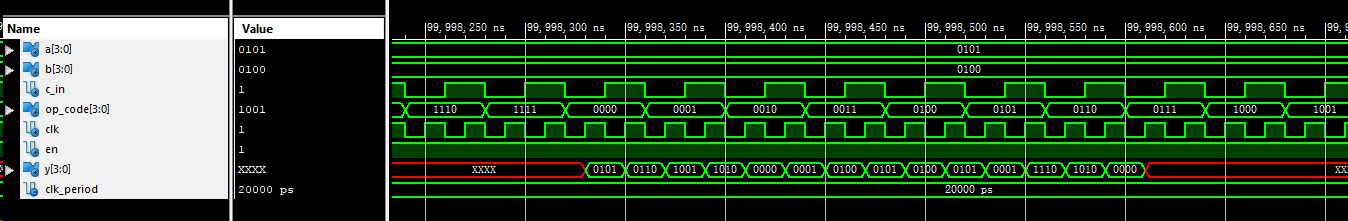
\includegraphics[width=1\linewidth]{homework6-1}
      \caption{The behaviour simulation result (2)}
      \label{fig:homework6-1}
    \end{figure}

    \begin{figure}
      \centering
      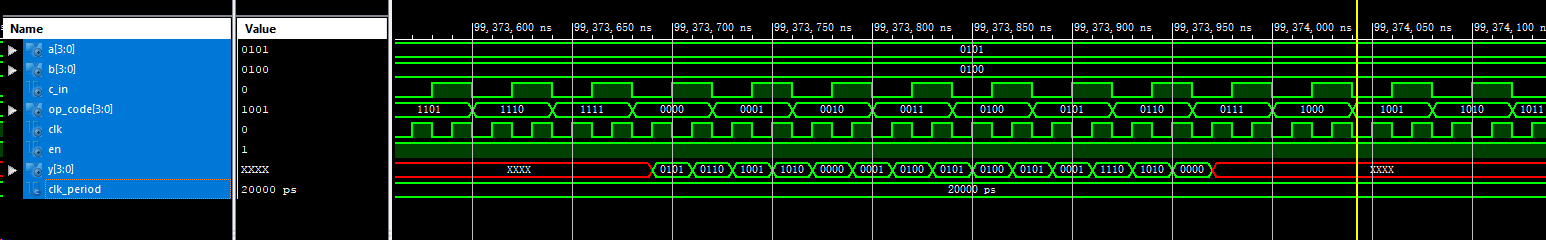
\includegraphics[width=1\linewidth]{homework6-2}
      \caption{The behaviour simulation result (1)}
      \label{fig:homework6-2}
    \end{figure}

    The result of the both are same, and those are, in order, "0101","0110","1010","1110","1010","XXXX".

    And the source of the test bench is the following.

\begin{lstlisting}[language=VHDL]
library IEEE;
use IEEE.STD_LOGIC_1164.ALL;
use IEEE.STD_LOGIC_ARITH.all;
use IEEE.STD_LOGIC_UNSIGNED.all;

ENTITY alu_tb IS
END alu_tb;
 
ARCHITECTURE behavior OF alu_tb IS 
 
    -- Component Declaration for the Unit Under Test (UUT)  
    COMPONENT alu
    PORT(
         Y : OUT  std_logic_vector(3 downto 0);
         A : IN  std_logic_vector(3 downto 0);
         B : IN  std_logic_vector(3 downto 0);
         C_IN : IN  std_logic;
         OP_CODE : IN  std_logic_vector(3 downto 0) ;
         CLK : IN  std_logic;
         EN : IN  std_logic
        );
    END COMPONENT;
    
   --Inputs
   signal A : std_logic_vector(3 downto 0) := "0101";
   signal B : std_logic_vector(3 downto 0) := "0100";
   signal C_IN : std_logic := '0';
   signal OP_CODE : std_logic_vector(3 downto 0) := (others => '1');
   signal CLK : std_logic := '0';
   signal EN : std_logic := '0';

   --Outputs
   signal Y : std_logic_vector(3 downto 0);

   -- Clock period definitions
   constant CLK_period : time := 10 ns;
 
BEGIN 
	-- Instantiate the Unit Under Test (UUT)
   uut: alu PORT MAP (
          Y => Y,
          A => A,
          B => B,
          C_IN => C_IN,
          OP_CODE => OP_CODE,
          CLK => CLK,
          EN => EN
        );

   -- Clock process definitions
   CLK_process :process
   begin
		CLK <= '0';
		wait for CLK_period/2;
		CLK <= '1';
		wait for CLK_period/2;
   end process;
 
	-- enable process
	enable_proc: process
	begin
		-- hold off EN  for 10 clk period
      wait for 10*CLK_period;	
		EN <= '1';
		wait;
	end process;
	
	-- op_code process
	op_proc: process
	begin
		-- change operation code for every two clock tick.
		wait for 2*CLK_period;
		if (EN = '1') then
			OP_CODE <= OP_CODE + 1;
		end if;
	end process;
	
	-- carry process
	carry_process: process
	begin
		-- change carry state each clock tick.
		wait for CLK_period;
		c_in <= '1';
		wait for CLK_period;
		c_in <= '0';
	end process;
END;
\end{lstlisting}

    \section{Post-Route Simulation}
    \label{sec:simu:post}
    
    Those test datas will be used continued. But the differences are the delays of the signals.
    For the basic test and verification, the frequency is 100MHz.

    The result of the one with case-when notion is the figure \ref{fig:homework6-3}, and the detail 
    of the delay is the figure \ref{fig:homework6-4}. The delay between the "do" signal of the clock
    -- the rising edge, is ``huge'', and the result ``come out'' after more than half of the clock period. 
    The result of the one with with-select notion is the figure \ref{fig:homwork6-5}, and the detail
    of the delay is the figure \ref{fig:homework6-6}. The delay in the result is also ``huge''.

      \begin{figure}
        \centering
        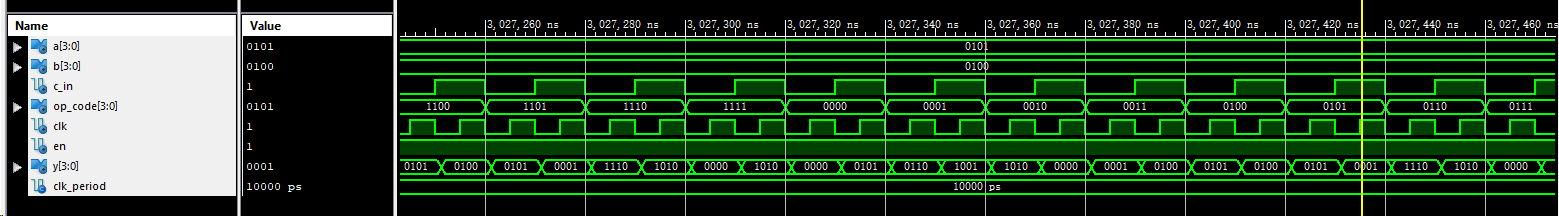
\includegraphics[width=1\linewidth]{homework6-3}
        \caption{The post-route simulation result (1)}
        \label{fig:homework6-3}
      \end{figure}

      \begin{figure}
        \centering
        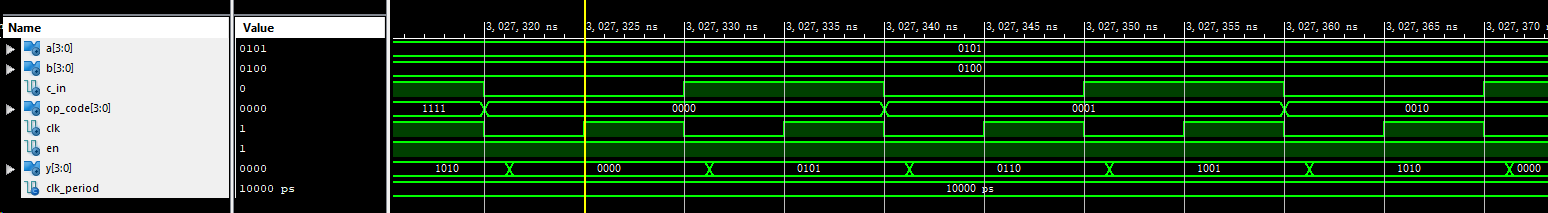
\includegraphics[width=1\linewidth]{homework6-4}
        \caption{The post-route simulation result (2)}
        \label{fig:homework6-4}
      \end{figure}

      \begin{figure}
        \centering
        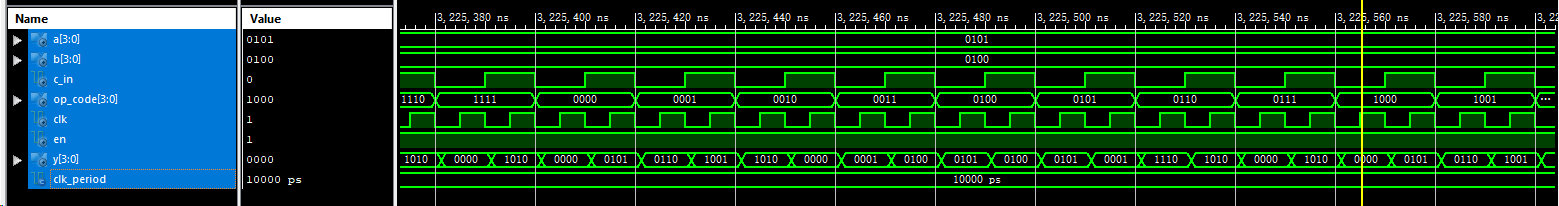
\includegraphics[width=1\linewidth]{homework6-5}
        \caption{The post-route simulation result (3)}
        \label{fig:homework6-5}
      \end{figure}

      \begin{figure}
        \centering
        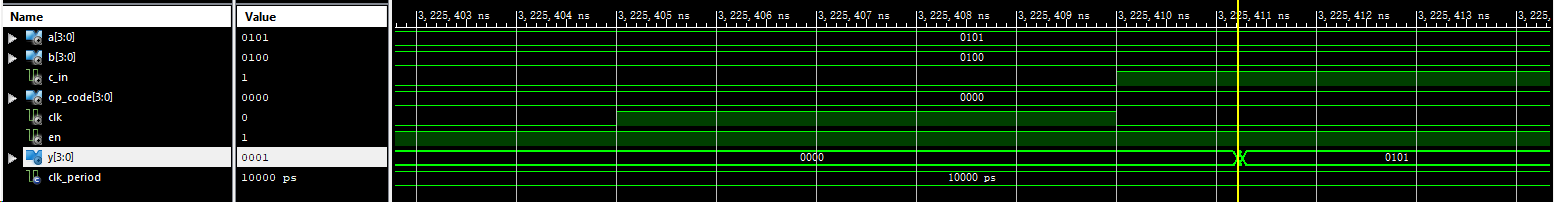
\includegraphics[width=1\linewidth]{homework6-6}
        \caption{The post-route simulation (4)}
        \label{fig:homework6-6}
      \end{figure}

      The highest frequency of the both kinds of the ALU is 100MHz, but that might be unstable.
      So the stable highest frequency of the kinds of the ALU is 50MHz, half of the 100Mhz.
      And the uesr might has the change to overclock.

      \section{RTL Schematics and Implemented Summary}
      \label{sec:rsnis}

\begin{figure}
\centering
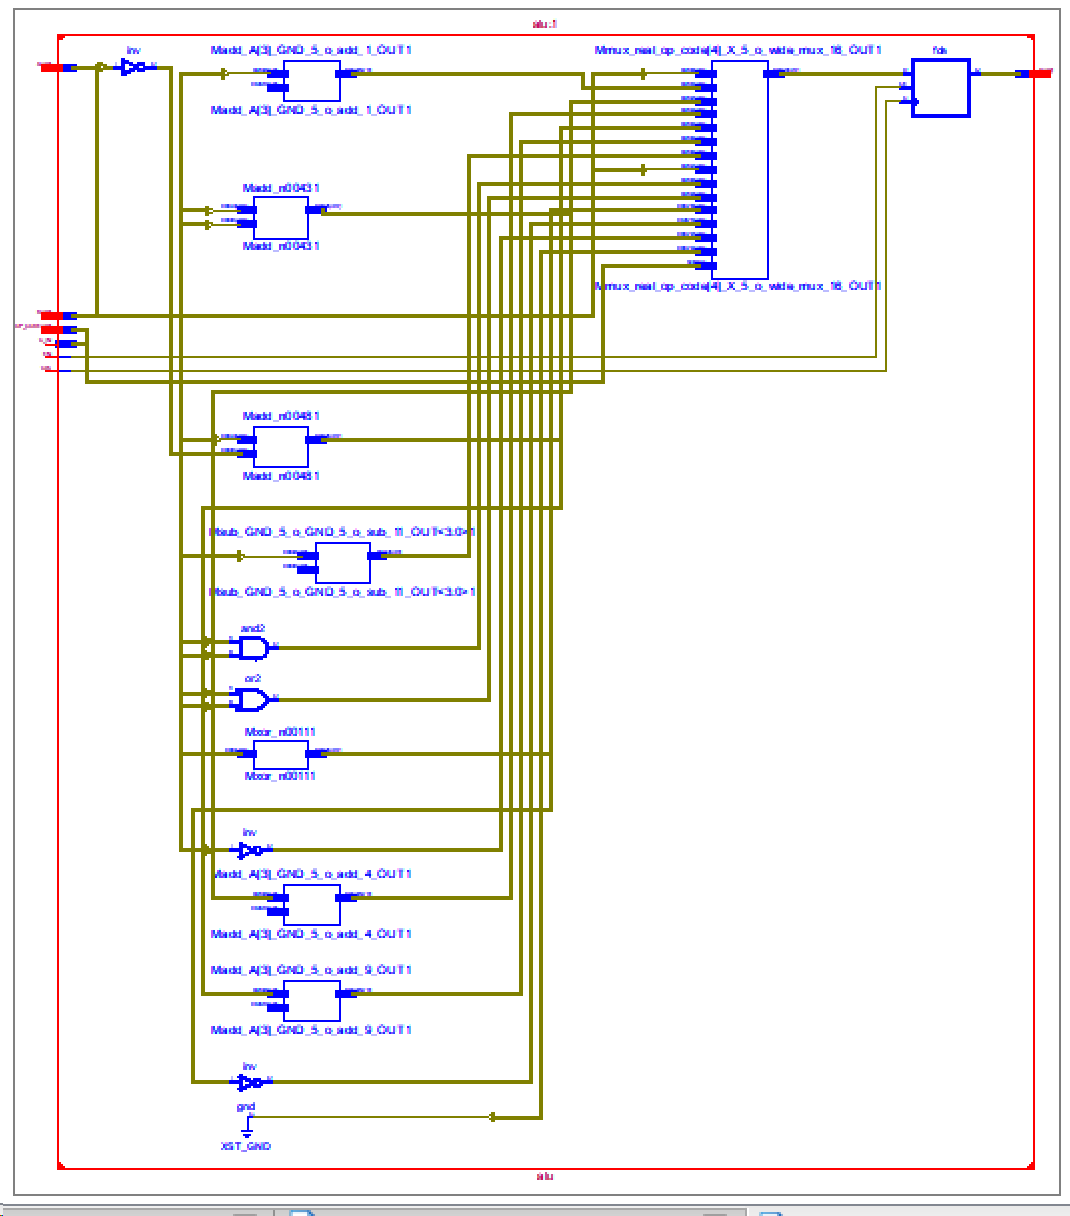
\includegraphics[width=1\linewidth]{homework6-8}
\caption{The RTL Schematic of ALU (1)}
\label{fig:homework6-8}
\end{figure}


    \begin{figure}
      \centering
      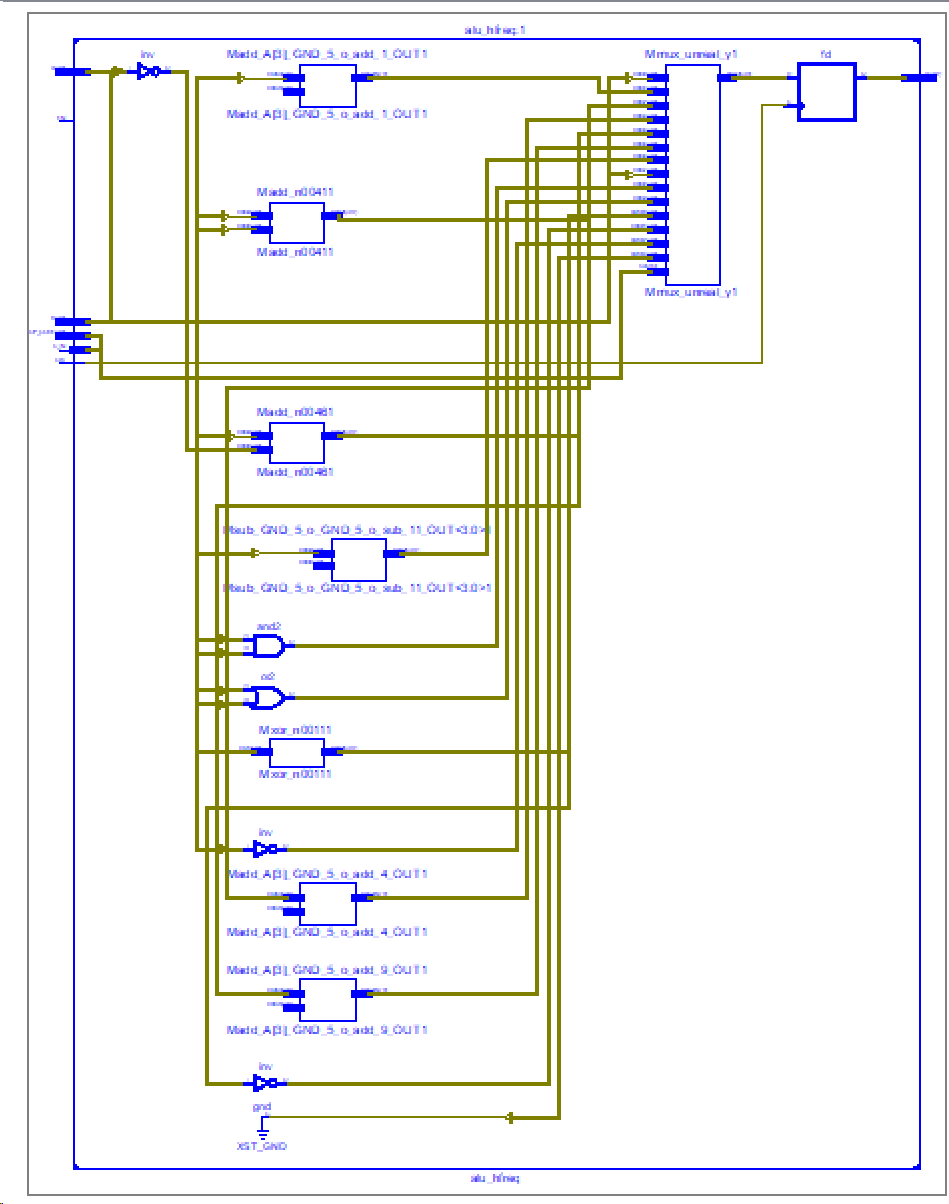
\includegraphics[width=1\linewidth]{homework6-7}
      \caption{The RTL Schematic of ALU (2)}
      \label{fig:homework6-7}
    \end{figure}
    

    The RTL schematics of the ALU are the figure \ref{fig:homework6-8} and the figure \ref{fig:homework6-7}.
    
   
\end{document}